\section{Results}
\label{sec:results}
Directional shrinkage meets the prespecified success criterion on TCGA-UT and fails it on BRACS. On TCGA-UT, the tuned arm gains 1.29 points at five patients (95\% interval: 0.99 to 1.57), the fixed arm 1.03 points (0.83 to 1.22), and both gains shrink with the patient count, to 0.41 and 0.21 points at twenty (Table~\ref{tab:accuracy}). On BRACS, the tuned arm gains 0.36 points at five patients ($-0.31$ to 1.11), the fixed arm 0.69 ($-0.33$ to 1.76), and at twenty patients both are slightly negative. The primary contrast therefore succeeds on one dataset only, and no claim across both cohorts is supported.

\begin{table}[htbp]
\centering
\small
\renewcommand{\arraystretch}{1.15}
\begin{tabular}{@{}lrrr@{}}
\toprule
Arm family & $G=5$ & $G=10$ & $G=20$ \\
\midrule
\multicolumn{4}{@{}l}{\emph{TCGA-UT}}\\
Real (R) & 62.48 [61.24, 63.65] & 67.79 [66.47, 69.00] & 71.89 [70.55, 73.06] \\
Directional, closed form (A) & 63.51 [62.24, 64.67] & 68.27 [66.95, 69.45] & 72.10 [70.76, 73.28] \\
Directional, tuned (At) & 63.77 [62.51, 64.90] & 68.50 [67.20, 69.67] & 72.30 [70.98, 73.45] \\
Pool centres (C) & 73.14 [71.62, 74.50] & 74.47 [73.01, 75.78] & 75.55 [74.11, 76.85] \\
\addlinespace
Gain A $-$ R & 1.03 [0.83, 1.22] & 0.48 [0.39, 0.57] & 0.21 [0.16, 0.25] \\
Gain At $-$ R & \textbf{1.29} [0.99, 1.57] & 0.71 [0.52, 0.90] & 0.41 [0.28, 0.54] \\
Headroom C $-$ R & 10.66 [9.78, 11.47] & 6.68 [5.94, 7.42] & 3.66 [3.06, 4.30] \\
\addlinespace
\multicolumn{4}{@{}l}{\emph{BRACS}}\\
Real (R) & 36.18 [33.46, 38.80] & 38.49 [35.87, 41.22] & 40.97 [38.50, 43.62] \\
Directional, closed form (A) & 36.87 [34.45, 39.27] & 38.86 [36.34, 41.47] & 40.63 [37.97, 43.50] \\
Directional, tuned (At) & 36.54 [34.02, 39.11] & 38.84 [36.32, 41.47] & 40.85 [38.18, 43.62] \\
Pool centres (C) & 44.63 [41.33, 48.05] & 45.11 [41.85, 48.51] & 45.50 [42.20, 48.76] \\
\addlinespace
Gain A $-$ R & 0.69 [$-0.33$, 1.76] & 0.37 [$-0.46$, 1.17] & $-0.35$ [$-1.34$, 0.55] \\
Gain At $-$ R & \textbf{0.36} [$-0.31$, 1.11] & 0.34 [$-0.29$, 1.01] & $-0.12$ [$-0.92$, 0.63] \\
Headroom C $-$ R & 8.45 [6.31, 10.84] & 6.61 [4.85, 8.58] & 4.53 [2.77, 6.37] \\
\bottomrule
\end{tabular}
\caption{Directional shrinkage gains about one point at five TCGA-UT patients and nothing distinguishable from zero on BRACS. Accuracy entries are test patient-macro balanced accuracy in percent; gains and headroom are paired contrasts in percentage points; bold entries are the primary contrast. Intervals are 95\% bootstrap intervals over test patients and draws. The R and C rows are those of \citet{queisler2026centreError} and \citet{queisler2026bracsMechanism}.}
\label{tab:accuracy}
\end{table}

\noindent The TCGA-UT success is narrow in two respects. Its point estimate clears the one-point threshold, but the lower interval bound of 0.99 does not, so the data exclude a zero gain but not a gain slightly below the threshold. And the gain is small against the headroom: at five patients the tuned arm captures 12 percent of what correct centres are worth.

\subsection{Headroom recovery and the patient-count gap}
\label{sec:recovery-results}
On TCGA-UT, the tuned arm recovers 0.121 (0.093 to 0.148) of the pool-centre headroom at five patients and 0.106 (0.078 to 0.135) at ten; the fixed arm recovers 0.097 and 0.071 (Table~\ref{tab:shares}). These are the first cohort-only centre corrections in this series with recovery intervals clearly above zero on TCGA-UT, where radial shrinkage recovered $-0.028$ and 0.024. The gain decays with the patient count roughly as the headroom does, so the five-to-twenty gap narrows from 9.41 to 8.53 points, a shrinkage share of 0.09 (0.06 to 0.12). On BRACS, recovery is 0.043 ($-0.041$ to 0.124) at five patients and 0.052 at ten, and the gap share of 0.10 ($-0.12$ to 0.29) is indistinguishable from zero.

\begin{table}[htbp]
\centering
\small
\renewcommand{\arraystretch}{1.15}
\begin{tabular}{@{}lrr@{}}
\toprule
 & TCGA-UT & BRACS \\
\midrule
Recovery $\rho_5$, A & 0.097 [0.077, 0.116] & 0.082 [$-0.045$, 0.191] \\
Recovery $\rho_5$, At & 0.121 [0.093, 0.148] & 0.043 [$-0.041$, 0.124] \\
Recovery $\rho_{10}$, A & 0.071 [0.059, 0.086] & 0.056 [$-0.071$, 0.180] \\
Recovery $\rho_{10}$, At & 0.106 [0.078, 0.135] & 0.052 [$-0.049$, 0.153] \\
\addlinespace
Gap, real $\Delta^{\mathrm R}_{5\to20}$ & 9.41 [8.71, 10.12] & 4.80 [2.88, 6.75] \\
Gap, tuned $\Delta^{\mathrm{At}}_{5\to20}$ & 8.53 [7.82, 9.24] & 4.31 [2.48, 6.07] \\
Share, A, $5\to20$ & 0.09 [0.07, 0.11] & 0.22 [$-0.03$, 0.46] \\
Share, At, $5\to10$ & 0.11 [0.05, 0.16] & 0.01 [$-0.48$, 0.35] \\
Share, At, $10\to20$ & 0.07 [0.03, 0.11] & 0.19 [$-0.24$, 0.54] \\
Share, At, $5\to20$ & 0.09 [0.06, 0.12] & 0.10 [$-0.12$, 0.29] \\
\bottomrule
\end{tabular}
\caption{On TCGA-UT directional shrinkage captures a tenth of the pool-centre headroom and removes a tenth of the patient-count gap; on BRACS neither quantity is distinguishable from zero. Recovery is the gain divided by the headroom at the same patient count; the share is the fraction of the real patient-count gap that the shrunk arms remove. Gaps are in percentage points. The BRACS ratios divide noisy differences estimated on 24 test patients per split and should be read only as bounds.}
\label{tab:shares}
\end{table}

\subsection{Comparison with the other cohort-only remedies}
\label{sec:comparison-results}
Against radial shrinkage, directional shrinkage is better on TCGA-UT at every patient count and worse on BRACS (Figure~\ref{fig:gains}). On TCGA-UT, At exceeds tuned radial shrinkage by 1.14 points at five patients (0.84 to 1.43), 0.57 at ten, and 0.27 at twenty, all with intervals above zero. On BRACS, it falls behind tuned radial shrinkage by 0.62 points at five patients ($-1.47$ to 0.15) and 0.61 at twenty, and behind the closed-form radial arm by 0.87 points at twenty ($-1.70$ to $-0.03$). The two datasets thus reverse the ranking of the two first-moment estimators.

Cohort whitening remains the stronger remedy on TCGA-UT. It gains 2.26, 1.85, and 1.27 points at five, ten, and twenty patients, so At trails it by 0.97 ($-1.21$ to $-0.74$), 1.15, and 0.86 points. On BRACS, where cohort whitening gains nothing measurable, At and RWc are indistinguishable (0.05 points at five patients, $-0.68$ to 0.66). On TCGA-UT, directional shrinkage thus closes about half of the distance between radial shrinkage and cohort whitening at five patients, and a quarter to a third at ten and twenty, without overtaking whitening anywhere.

\begin{figure}[htbp]
\centering
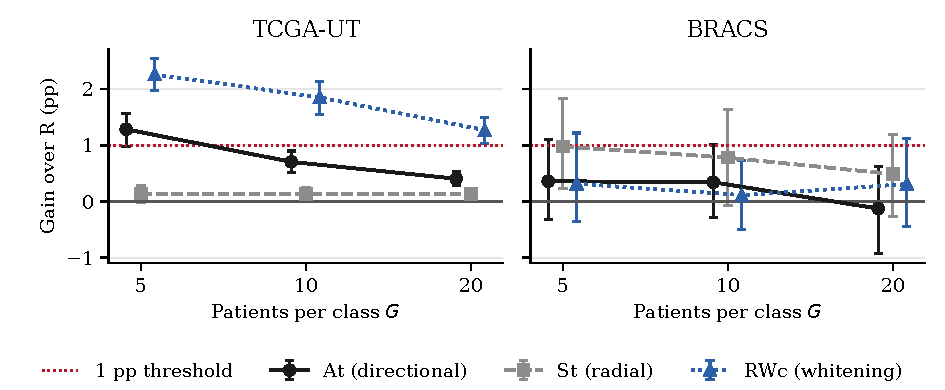
\includegraphics[width=\textwidth]{gains_by_patient_count.pdf}
\caption{Directional shrinkage sits between radial shrinkage and cohort whitening on TCGA-UT and is indistinguishable from zero on BRACS. Paired gains over the real cohort in percentage points; error bars show the paired 95\% bootstrap intervals. Only the TCGA-UT five-patient At point clears the one-point threshold.}
\label{fig:gains}
\end{figure}

\subsection{Selected strengths and basis rank}
\label{sec:alpha-results}
Validation selection behaves differently on the two datasets (Table~\ref{tab:alpha}). On TCGA-UT it never selects $\alpha=0$ and moves to stronger shrinkage as the patient count grows: the closed-form strength or twice it at five patients, $\alpha=2$ in 27 of 30 fits at ten, and $\alpha=2$ or the grid maximum $\alpha=4$ at twenty, where 12 of 30 fits sit on the upper boundary. On BRACS, $\alpha=0$ is chosen in 5 to 9 of 30 fits per patient count and the halved strength is the most frequent or joint most frequent choice, so the validation data often prefer weak shrinkage or none.

\begin{table}[htbp]
\centering
\small
\renewcommand{\arraystretch}{1.15}
\begin{tabular}{@{}llrrrrrr@{}}
\toprule
Dataset & $G$ & Rank & $\alpha=0$ & 0.5 & 1 & 2 & 4 \\
\midrule
TCGA-UT & 5 & 120 & 0 & 0 & 14 & 12 & 4 \\
        & 10 & 270 & 0 & 1 & 1 & 27 & 1 \\
        & 20 & 570 & 0 & 0 & 0 & 18 & 12 \\
\addlinespace
BRACS & 5 & 28 & 9 & 12 & 5 & 2 & 2 \\
      & 10 & 63 & 8 & 10 & 7 & 5 & 0 \\
      & 20 & 133 & 5 & 10 & 10 & 5 & 0 \\
\bottomrule
\end{tabular}
\caption{TCGA-UT validation data favour strong directional shrinkage; BRACS validation data favour weak shrinkage or none. Counts are tuned classifiers out of 30 per dataset and patient count (three splits, ten draws). The rank is that of the cohort's pooled between-patient covariance, which equals its maximum $C(G-1)$ in every draw.}
\label{tab:alpha}
\end{table}

\noindent The covariance rank is always full, so the eigenbasis spans 120 to 570 of the 2,560 feature dimensions on TCGA-UT and 28 to 133 on BRACS. On BRACS at five patients, a third of the eigen-directions have no estimated separation beyond noise ($s_j=0$) and are shrunk completely at $\alpha=1$; on TCGA-UT fewer than one in a hundred are.

\subsection{What the directional correction changes}
\label{sec:geometry-results}
A diagnostic on the exact fitted cohorts, computed after all fits were locked, compares each estimator's centres with the pool centres (Table~\ref{tab:geometry}). Following \citet{queisler2026centreError}, it splits the squared centre error into a part shared by all classes, a class-specific part inside the $(C-1)$-dimensional discriminant subspace spanned by the centred pool centres, and a class-specific part outside it. Directional shrinkage preserves the grand mean, so it cannot change the shared part.

\begin{table}[htbp]
\centering
\small
\renewcommand{\arraystretch}{1.15}
\begin{tabular}{@{}llrrrrrrr@{}}
\toprule
 & & & & \multicolumn{3}{c}{$\Delta$ squared error} & \multicolumn{2}{c}{A: $\Delta$ by part} \\
\cmidrule(lr){5-7}\cmidrule(lr){8-9}
Dataset & $G$ & $\bar a$ & Off-span & A & At & S & Disc. & Off \\
\midrule
TCGA-UT & 5 & 0.41 & 0.26 & $-4\%$ & $+41\%$ & $-19\%$ & $+6\%$ & $-10\%$ \\
        & 10 & 0.19 & 0.15 & $-6\%$ & $+33\%$ & $-10\%$ & $+5\%$ & $-10\%$ \\
        & 20 & 0.10 & 0.11 & $-3\%$ & $+62\%$ & $-3\%$ & $+5\%$ & $-8\%$ \\
\addlinespace
BRACS & 5 & 0.78 & 0.39 & $-4\%$ & $-6\%$ & $-26\%$ & $+10\%$ & $-14\%$ \\
      & 10 & 0.58 & 0.34 & $+4\%$ & $+5\%$ & $-8\%$ & $+19\%$ & $-16\%$ \\
      & 20 & 0.45 & 0.35 & $+15\%$ & $+13\%$ & $+8\%$ & $+25\%$ & $-10\%$ \\
\bottomrule
\end{tabular}
\caption{Directional shrinkage barely reduces centre error, and the tuned strength on TCGA-UT increases it. $\bar a=\sum_j n_ja_j/\sum_j n_j$ is the noise-weighted mean weight at $\alpha=1$. Off-span is the fraction of the squared correction $\sum_c\lVert\tilde{\boldsymbol\mu}_c-\hat{\boldsymbol\mu}_c\rVert^2$ at $\alpha=1$ that lies outside the span of the cohort's centred class centres. $\Delta$ squared error is the relative change of $\sum_c\lVert\cdot-\boldsymbol\mu_c^{\mathrm{pool}}\rVert^2$ against the raw cohort centres, for the closed-form arm (A), the tuned arm at its selected strength (At), and closed-form radial shrinkage (S). The last two columns split the change of arm A into its discriminant and off-discriminant parts, as percentages of the raw squared error. Values are means over three splits and ten draws.}
\label{tab:geometry}
\end{table}

\noindent In one respect the estimator does what its construction promises. A quarter of its correction at five TCGA-UT patients, and 39 percent on BRACS, lies outside the span of the cohort's own class centres, the region that radial shrinkage cannot reach at all. Measured against the pool's geometry, it removes off-discriminant error worth 10 and 14 percent of the raw squared error at five patients. But it adds discriminant error of 6 and 10 percent in exchange, so the net reduction in squared centre error is only 4 percent on both datasets, a fifth of what radial shrinkage achieves. On BRACS the added discriminant error grows with the patient count, and the net change turns positive at ten patients.

The accuracy gains do not follow the centre error. On TCGA-UT at five patients, radial shrinkage removes 19 percent of the squared centre error and loses 0.30 points, closed-form directional shrinkage removes 4 percent and gains 1.03 points, and the tuned arm increases squared centre error by 41 percent and gains 1.29 points. At every patient count, the tuned arm's added error lies almost entirely inside the discriminant subspace, and it still gains the most. Across the 30 draws per patient count, the correlation between the gain of arm A and its reduction in squared centre error lies between 0.01 and 0.19 on TCGA-UT. Whatever the tuned arm improves, it is not the distance of the class centres from the pool centres.

One mechanism consistent with these observations is a first-moment analogue of whitening. Shrinking the class centres along the directions in which the cohort's patients vary most contracts class separation along exactly those directions. The classifier then has less reason to rely on them, which is what whitening along the cohort's between-patient basis achieves by rescaling the features \citep{queisler2026patientDirections}. On this reading, validation prefers strong shrinkage because it discards unreliable patient directions, not because it moves the centres closer to the truth. The reading also matches where the remedy works: 1.29 points on TCGA-UT, where cohort whitening gains 2.26, and nothing on BRACS, where cohort whitening also gains nothing. The fits do not test this reading directly; it is an interpretation of the diagnostic, not a measured decomposition.

\section{Discussion}
\label{sec:discussion}
Directional shrinkage is the first cohort-only centre correction in this series to clear the practical threshold on TCGA-UT, and it meets the prespecified criterion: 1.29 points at five patients, with an interval from 0.99 to 1.57. It recovers 12 percent of the pool-centre headroom, where radial shrinkage recovered none, and it narrows the five-to-twenty patient gap by 9 percent. On BRACS it recovers nothing measurable, and radial shrinkage remains the better estimator there. The result is therefore dataset-specific: success on TCGA-UT, a subthreshold and inconclusive effect on BRACS, and no support for a claim across cohorts.

The diagnostic changes what the TCGA-UT success means. The estimator was motivated as a better estimate of the class centres, yet its closed-form version reduces squared centre error only slightly and its tuned version increases it substantially. The gain is thus not evidence that a cohort can estimate its own class centres better from its own patients; on that question, the geometry here supports the conclusion of \citet{queisler2026centreShrinkage}. What the cohort can do is decide which directions of its class-centre configuration not to trust. That is a second-moment operation expressed through the first moment, and it behaves like the second-moment remedy: helpful on TCGA-UT, ineffective on BRACS, and weaker than cohort whitening itself.

Two practical conclusions follow. First, for a five-patient TCGA-UT cohort, cohort whitening remains the better cohort-only remedy, by about one point at every patient count. Whether the two remedies add up is not tested here, and the shared mechanism suggested above makes a large combined gain unlikely. Second, the centre-error headroom of eight to eleven points remains almost entirely unrecovered. Two cohort-only centre estimators have now been tested against it, and the better one recovers 12 percent on one dataset while leaving centre error nearly unchanged. This strengthens the conclusion that the missing centre information must come from outside the labelled cohort, for example from related classes, unlabelled slides, or a population covariance used as a prior.

\section{Limitations}
\label{sec:limitations}
The estimator pools the between-patient covariance across classes, which assumes that all classes share the same patient-level noise. The eigenbasis and its eigenvalues are estimated from $C(G-1)$ patient deviations in 2,560 dimensions, only 28 for BRACS at five patients, and the separation estimate $s_j$ uses $C-1$ degrees of freedom per direction, six on BRACS. Both estimates are noisy, and directions outside the estimated span, most of the feature space, are never shrunk. Weights that borrow strength across directions, or a covariance estimated outside the cohort, could behave differently.

The strength grid stops at $\alpha=4$, which 12 of 30 tuned fits at twenty TCGA-UT patients selected, so the tuned arm may be limited by the grid at that patient count. The grid was not extended after test results were inspected. The primary contrast is less affected: at five patients, 4 of 30 fits chose the boundary. The TCGA-UT lower interval bound of 0.99 points does not exclude a gain slightly below the practical threshold.

The geometric diagnostic uses the pool centres as the reference for the true class centres. These centres are themselves estimated from the eligible training patients of each split, so they carry sampling error and share patients with the cohorts. The diagnostic is descriptive and has no intervals, and its mechanistic reading in Section~\ref{sec:geometry-results} is an interpretation rather than a tested decomposition. All arms reuse the three evaluation splits of the source studies, so they share test patients with every earlier comparison in this series. The results are conditional on frozen Virchow2 features, multinomial logistic regression, 160 patches per class, and the two cohorts studied; transfer to other cohorts, feature extractors, or class counts is untested.
